\documentclass[tikz,border=2cm]{standalone}
% https://tex.stackexchange.com/questions/734715/how-to-draw-the-shadow-in-this-decoration-of-wrapped-tape-in-tikz
\begin{document}
\def\mydraw{%
    \draw[cyan] (O.north) -- (O.north west) arc (270:90:.05cm) -- ([xshift=.3cm,yshift=.1cm]O.north west) arc (270:450:.05cm) -- ++(-1.5cm,0) -- ([xshift=-.5cm,yshift=.1cm]O.west) -- ([xshift=-1.2cm,yshift=.1cm]O.south west) -- ([xshift=-.05cm,yshift=.1cm]O.south west);%
    \draw[magenta] ([yshift=.05cm,xshift=-.05cm]O.north west) -- ([xshift=-.05cm]O.south west) arc (180:270:.05cm) --([yshift=-.05cm]O.south);%
    \filldraw[fill=gray!50,draw=cyan] ([yshift=.15cm,xshift=.35cm]O.north west) -- ++(0,-.15cm) -- ++(-.35cm,0) arc (270:90:.05cm) -- ([xshift=.3cm,yshift=.1cm]O.north west) arc (270:360:.05cm);%
}
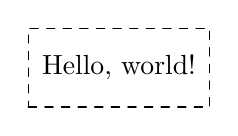
\begin{tikzpicture}[line cap=round]
    \node[minimum size=1cm,inner sep=5pt,style=dashed,draw] (O) {Hello, world!};
    \begin{scope}
         \mydraw
    \end{scope}
    \begin{scope}[transform canvas={xscale=-1}]
        \mydraw
    \end{scope}
\end{tikzpicture}
\end{document}